\section{Internet-scale analysis}
\label{sec:internet-scale}

In the preceding sections we have presented our \name attacks and evaluated
their effectiveness, but we have yet to understand what entities can mount them.
In this section, we aim to quantify the likelihood that any AS is in a position
to mount \name attacks.

\subsection{Approach}

Figure~\ref{fig:simulations} summarizes our simulation approach, which we detail
in the next section.  In short, we model the activity of Tor users and simulate
their path selection using TorPS~\cite{TorPS}.  TorPS returns guard and exit
relays, which we then feed as input---together with source ASes and destination
addresses---into our framework that runs traceroutes from RIPE Atlas nodes.  The
rest of this section describes our approach in detail.

\subsubsection{Attack model}

\begin{figure}[t]
	\centering
	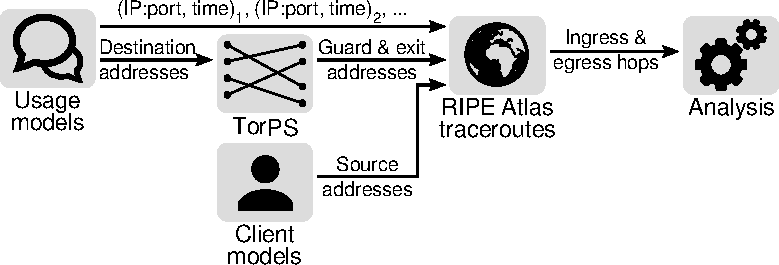
\includegraphics[width=\linewidth]{figures/simulations.pdf}
	\caption{The relation among our simulation components.  Our goal is to
	determine the ASes a Tor user's traffic traverses into and out of the Tor
	network.  Duplicate ASes on both sides can deanonymize streams.}
	\label{fig:simulations}
\end{figure}

We assume that an AS can mount \name attacks if it can see both traffic
\emph{entering} the Tor network and DNS traffic \emph{exiting} the Tor network.
Recall that an exit relay can perform DNS resolution in two ways; by running a
local resolver, or by relying on a third-party resolver, such as its ISP's or
Google's public resolver.  In the case of exit relays that perform local
resolution, an effective position for an attacker is both \first~anywhere on the
AS path between a Tor client and its guard relay; and \second~anywhere on the
path between an exit relay and any of the name servers the exit has to
communicate with to resolve a domain.  These name servers include the full DNS
delegation path, \ie, a root name server plus subsequent name servers in the DNS
hierarchy.  All ASes along the path from the exit relay to the name servers will
be able to see the domain names that the exit relay is querying.  For exit
relays that rely on third-party resolvers, the adversary instead has to be on
the path between the exit relay and its DNS resolver.
%)\fixme{QUESTION: ``In addition, the DNS queries will look like they are coming
%from the IP address of the name server and not the IP address of the
%exit relay.''--This new wording seems unclear to me now--wanted to say
%that ASes on the path from the 3rd-party to the DNS servers will see that
%the queries are coming from the 3rd-party and not the exit IP, which is
%why we ignore them . . .}

\subsubsection{Simulating Tor user activity with TorPS}

To measure the likelihood that an AS can be in a position to perform a \name
attack, we use TorPS~\cite{TorPS}---short for Tor Path Simulator---which mimics
how a Tor client constructs circuits (see ``TorPS'' in
Figure~\ref{fig:simulations}).  TorPS takes as input archived Tor network
data~\cite{collector} and usage models, which are sets of IP addresses that Tor
clients talk to---\eg web servers.  Given this input, TorPS then simulates for a
configurable number of ``virtual'' Tor clients the way they would select guard
and exit relays.  TorPS is based on the Tor stable release in version 0.2.4.23.
For each simulated client, TorPS uses one guard; this guard selection expires
after 270 days.  We use TorPS to simulate the behavior of 100,000 Tor clients
for the entire month of March 2016.

% \fixme{Wording, please: ``we perform 100,000 samples in the TorPS Monte Carlo
% simulation'' or ``we perform 100,000 Monte Carlo simulations in order to
% analyze this.''}
%potential Tor users and how the Tor client would have behaved.
%we perform 100,000 samples in the TorPS Monte Carlo
%simulation.

We need to place our simulated Tor clients into an AS (see ``Client models'' in
Figure~\ref{fig:simulations}).  We selected clients in major ISPs in the
top-five most popular countries of Tor usage according to Tor
Metrics~\cite{metrics-countries}.  As of August 2016, the top five countries are
the U.S., Russia, Germany, France, and the U.K.  For the U.S., we chose Comcast
(AS~7922); for Russia, Rostelecom (AS~42610); for Germany, Deutsche Telekom
(AS~3320); for France, Orange (AS~3215); and for the U.K., British Telecom
(AS~2856).

Having placed simulated Tor clients into ASes, we now model their activity over
Tor (see ``Usage models'' in Figure~\ref{fig:simulations}).  We model each
client to have visited several websites every day in March 2016.\footnote{We
modeled our client behavior off of the ``Typical'' model that Johnson
\ea~\cite[\S~5.1.2]{Johnson2013a} used.}  At 9 a.m. EST, the client visits {\tt
mail.google.com} and {\tt www.twitter.com}.  At 12 p.m. EST, the client visits
{\tt calendar.google.com} and {\tt docs.google.com}. At 3 p.m. EST, the client
visits {\tt www.facebook.com} and {\tt www.instagram.com}.  Finally, at 6 p.m.
EST, the client visits {\tt www.google.com}, {\tt www.startpage.com}, and {\tt
www.ixquick.com}, and at 6:20 p.m. EST, the client visits {\tt www.google.com},
{\tt www.startpage.com}, and {\tt www.ixquick.com} again. Each of the 100,000
simulated Tor clients thus had $12 \cdot 31 = 372$ opportunities to be
compromised given 31 days and 12 site visits per day.  TorPS provided a new
circuit every ten minutes, regardless of how many distinct connections the
client made to different sites; it did not provide a new circuit for different
websites if the client visited the group of sites within the same ten-minute
window.
% This behavior differs from the latest Tor
% Browser, which provides new circuit for each distinct website, even within the
% same ten-minute time interval.  Thus, our results will be conservative in this
% respect.

For simplicity, we assume that only one DNS request occurs every time a client
visits a site. For example, in our model, at 9 a.m. one DNS request will occur
for {\tt mail.google.com} and one DNS request will occur for {\tt
www.twitter.com}. At 6 p.m. three DNS requests will occur, and at 6:20 p.m.
those same three DNS requests will occur again.   For now, we do not take
embedded requests (\ie for embedded website content such as YouTube videos) or
caching into account.
%\xxx{Shouldn't each
%  website actually result in hundreds of DNS lookups? This process could
%be more clear.}

\subsubsection{Inferring AS-level paths using traceroutes and {\tt pyasn}}

Our Internet-scale analysis also requires learning the AS-level paths from each
client to its guard, and from its exit to the destination (see ``RIPE Atlas
traceroutes'' in Figure~\ref{fig:simulations}).  We decided against the commonly
applied AS path inference because Juen \ea showed that it can be quite
inaccurate~\cite{Juen2015a}.  Traceroutes, in contrast, yield significantly more
accurate paths, but are difficult to run from Tor relays:  Past work involved
asking relay operators to run traceroutes for the
researchers~\cite[\S~4]{Juen2015a}.  This approach yielded traceroutes from
relays representing 26\% of exit bandwidth, but does not scale well.  Instead of
running traceroutes from Tor relays, we leverage the RIPE Atlas~\cite{atlas}
platform, a volunteer-run network measurement platform consisting of thousands
of lightweight and geographically spread \emph{probes} that can be used as
vantage points for traceroutes.  Our key observation is that RIPE Atlas has
probes in many ASes that also have Tor relays.  We leverage this observation by
designing measurements to run traceroutes from Atlas probes that are located in
the same AS as exit relays, to each of the destinations in question.

Table~\ref{tab:atlas-coverage} shows that for a day in May 2016, we found that
RIPE Atlas had probes in 52\% of ASes that contain exit relays, and in 51\% of
ASes that contain Tor guard relays.  More importantly, we found that Atlas ASes
cover 58\% of exit \emph{bandwidth} and 74\% of guard bandwidth.  This statistic
is important given that Tor clients select relays weighted by their bandwidth,
and the bandwidth of Tor relays is not uniformly distributed.  Given the growth
of both Tor and Atlas, we expect these numbers to increase in the future.  In
addition to Atlas, we also considered using PlanetLab~\cite{planetlab} to
initiate traceroutes, but unfortunately most PlanetLab nodes are located in
research and education networks~\cite{Banerjee2004a}, and are thus not
well-suited for performing our measurements.

% - 197 out of all 377 (52%) Tor exit ASes have Atlas probes.
% - 220 out of all 434 (51%) Tor guard ASes have Atlas probes.
% - Atlas ASes cover 57.53% of Tor exit bandwidth.
% - Atlas ASes cover 73.59% of Tor guard bandwidth.
\begin{table}[t]
	\renewcommand{\tabcaptext}{The coverage of RIPE Atlas nodes that are
	co-located with Tor guard and exit relays as of May 2016.}
	\topcap{\tabcaptext}
	\centering
	\begin{tabular}{l|r r}
	\toprule
	\textbf{Atlas probe coverage} & \textbf{Tor guard ASes} & \textbf{Tor exit ASes} \\
	\midrule
	By bandwidth & 73.59\% & 57.53\% \\
	By number & 50.69\% & 52.25\% \\
	\bottomrule
	\end{tabular}
	\bottomcap{\tabcaptext}
	\label{tab:atlas-coverage}
\end{table}

We performed traceroutes from the five Tor client ASes outlined above to all
their respective guard relay IP addresses that TorPS determined.  To measure the
paths from exit relays to their DNS resolvers, we performed the following
traceroutes, simulating four different DNS configurations:
\begin{itemize}
	\item \emph{ISP DNS:} To investigate the scenario in which an exit relay
		uses its ISP's resolver, we chose to represent this as the resolver
		being in the same AS as the exit relay.  Thus, no traceroutes were
		necessary for this experiment.  We acknowledge that this is not
		necessarily the case, but assume that it holds for the majority of exit
		relays.
		%To measure the path from an exit relay to its ISP's DNS resolver, we
		%perform traceroutes from a RIPE Atlas node in the ISP of the exit relay
		%to the ISP's corresponding DNS resolver.

	\item \emph{Google DNS:} This scenario represents an exit relay using
		Google's public resolver.  To measure the AS path, we perform
		traceroutes from a RIPE Atlas node in the AS of the exit relay to
		Google's public DNS resolver, \ie, {\tt 8.8.8.8}.

	\item \emph{Local DNS:} To measure the paths that would be traversed if an
		exit relay were running its own, local resolver (\eg, the popular
		service {\tt unbound}), we used the command line tool {\tt dig} with the
		{\tt +trace} option to determine the iterative resolution process.  We
		tracked all name server IP addresses from referrals at each level of the
		delegation path, and performed traceroutes to those IP addresses.

	\item \emph{Status quo:} This scenario represents the state of the Tor
		network as of March 2016, a combination of the above configurations.
		Recall that in Section~\ref{sec:mapping-resolvers}, we determined
		the IP addresses of the resolvers that exit relays use.  We ran
		traceroutes to these very IP addresses.  For the exit relays that used
		several resolvers during March, we randomly assigned one to the relay.
		We ended up having data for 73\% of the exit relays that TorPS ended up
		picking.\footnote{The missing 27\% are due to the churn in exit relays.
		Since we did not run our {\tt exitmap} experiment each hour, we were
		bound to miss some exit relays.}
\end{itemize}

We then mapped each IP address in every traceroute to its corresponding AS (see
``Analysis'' in Figure~\ref{fig:simulations}).  The
Python module {\tt pyasn}~\cite{pyasn} relies on BGP routing tables to perform
these mappings; by using a routing table that coincides with the time when we
performed our traceroutes, we can obtain accurate AS-level mappings.  This
method is subject to inaccuracies due to BGP route hijacks or leaks, but we
expect those events to be relatively unlikely for the time period and IP
prefixes that we are concerned with.

\subsubsection{Putting it all together}
Like Johnson \ea~\cite[\S~4.2]{Johnson2013a}, we consider two security metrics;
we aim to estimate \first the fraction of compromised streams per simulated Tor
user, and \second the amount of time it would take for the first compromise to
occur.  For both metrics, we consider the four DNS configurations outlined
above.  Our simulation can reveal the respective average threat that a given DNS
configuration poses for Tor users.

The traceroutes described in the previous section yielded two sets of ASes, one
from the Tor users' ASes to their guard relays, and one from approximately half
of the exit relays' ASes to the different destinations, which depend on the exit
relays' DNS configurations.  We intersect both AS sets (the ``ingress'' and
``egress'' hops of Figure~\ref{fig:simulations}) and classify a website visit as
compromised if the intersection is non-empty.  As stated earlier, for some exit
relays we did not have associated AS-level paths to a particular destination,
either due to a lack of co-located RIPE Atlas probes, or because of missing
traceroute information.  In these cases, we checked if the exit AS had the
potential to launch an attack, and if not, the stream was considered to be
uncompromised in order to err on the conservative side.
%we first searched for AS compromises between the ingress
%AS-level path and the AS of the exit relay (just like the \emph{ISP DNS} configuration
%above), and if there was no compromise, the stream is considered  before treating that
%particular stream as having not been compromised in order
%to err on the conservative side.

To compute the fraction of compromised streams, we counted the streams that were
compromised for every simulated user out of a possible maximum of 372. To
compute the time until first compromise, we determined the first stream in which
the user was compromised, took its timestamp, and calculated the offset from the
beginning of March 1, 2016.  For users that were not compromised during the
month of March, we assigned a maximum value of 31 days as the time until first
compromise, which is reflected in the plots in our next section.  Users who were
compromised immediately would have a value of 0, signifying that they were
compromised at the very beginning of March 1.

\subsection{Results}

\begin{figure}[t]
\centering
\subfigure[The fraction of compromised streams of simulated Tor clients.]{
	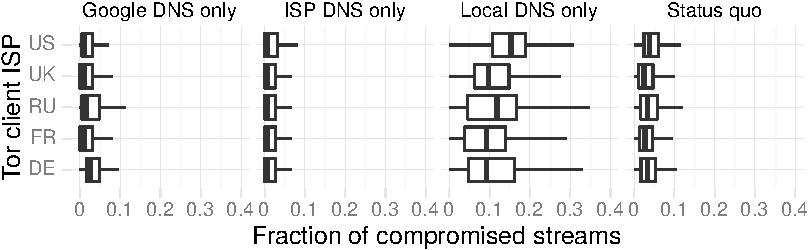
\includegraphics[width=\linewidth]{figures/compromised-streams.pdf}
	\label{fig:compromised-streams}
}
\subfigure[The time until simulated Tor clients got first compromised.]{
	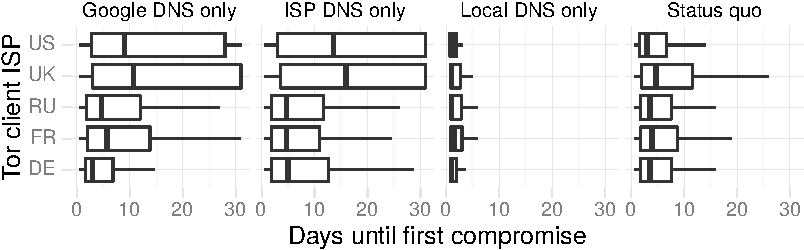
\includegraphics[width=\linewidth]{figures/time-until-compromise.pdf}
	\label{fig:time-until-compromise}
}
\caption{The fraction of compromised streams and the time until first compromise
for our simulated Tor clients.  We placed these clients in five popular client
ASes in the U.S., the U.K., Russia, France, and Germany.  For exit relays, we
consider the status quo (on the very right) plus three hypothetical DNS
configurations for all exit relays.  We do not plot outliers beyond the box
plots' whiskers.  In both experiments, the safest configuration is ``ISP DNS
only,'' \ie have all exit relays use their ISP's DNS resolver.}
\end{figure}

Figures~\ref{fig:compromised-streams} and~\ref{fig:time-until-compromise}
illustrate our results as box plots.  Each figure contains four subfigures, one
for each DNS configuration.  Each box plot contains five rows, one for each Tor
client AS.  For clarity, we did not plot any outliers beyond the box whiskers.

Both figures show that the ``ISP DNS only'' setup is the safest for Tor users,
\ie, it exhibits on average the least number of compromised streams while also
on average counting the most days until compromise.  This setup is closely
followed by ``Google DNS only,'' the status quo, and finally ``Local DNS only,''
which fares worse than all other setups.  We expected ``ISP DNS only'' to do
best because if all exit relays use their ISP's resolvers, there is only one AS
to contend with on the egress side---the exit relay's.  The Google setup fares
similarly well most likely because of Google's heavily anycast infrastructure
which minimizes the number of AS hops.  The status quo does significantly better
than the ``Local DNS'' results, presumably because only around 12\% of Tor exit
relays actually do their own resolution.  The wide variance observed in
Figure~\ref{fig:time-until-compromise} for ``ISP DNS'' and ``Google DNS'' is due
to using 31 days as a placeholder for simulated clients who were never
compromised.  However, a safe configuration against AS-level adversaries, which
our figures capture, is not necessarily the best setup for Tor users.  For
example, ISP-provided DNS resolvers can be misconfigured, subject to censorship,
or simply be a forwarder to Google's resolver, which already serves numerous
exit relays and whose centralization poses a threat to the anonymity of Tor
users.  We will explore this trade-off in greater detail in
Section~\ref{sec:discussion}.

Interestingly, we find differences in our five client ASes.  These differences
are particularly striking in Figure~\ref{fig:time-until-compromise}.  %For
%example, for ``Google DNS only'' and ``ISP DNS only,''  the median time until
%compromise differs by more than 10 days between UK, and RU or FR.  In general,
%UK and US users are doing better than users in RU, FR, and DE for these two
%setups.  
For example, for ``Google DNS only,'' the median time until compromise 
differs by around X days between DE and UK and around X days between 
DE and FR. For ``ISP DNS only,'' the median time until compromise differs by 
around X days between US and DE and around X days between US and FR.  
We conclude that the location of Tor clients matters and should be
considered in future traffic correlation studies.
